\section{Auswertung}
\label{sec:Auswertung}

\subsection{Fehler}
Für die Auswertung wird die \texttt{Python}-Bibliothek \texttt{numpy} \cite{numpy} benutzt. Die Fits entstehen mit \texttt{curve\_fit} aus \texttt{scipy.optimize} \cite{scipy}.
Die Fehlerrechnung wird mit \texttt{uncertainties} \cite{uncertainties} durchgeführt. Plots entstehen mit \texttt{matplotlib.pyplot} \cite{matplotlib}. \\
Der Mittelwert $\bar{x}$ von $N$ gemessenen Werten $a$ bestimmt sich über
\begin{equation}
    \bar{x} = \frac{1}{N} \sum^N_{i=1} a_i,
    \label{eq:mittelwerte}
\end{equation}
der Fehler des Mittelwertes über
\begin{equation}
    \Delta x = \sqrt{\frac{1}{N \cdot (N-1)} \sum^N_{i=1}(a_i - \bar{x})}.
    \label{eq:mittelwerte_fehler}
\end{equation}
Die Gaußsche Fehlerfortpflanzung für eine berechnete Größe $f$ lautet
\begin{equation}
    \Delta f = \sqrt{ \sum^N_{i=1} \left( \frac{\delta f}{\delta x_i}\right)^2 \cdot (\Delta x_i)^2}.
\end{equation}
Prozentuale Abweichungen werden mit
\begin{equation}
    \Delta x = \left|\frac{x - a}{a}\right|
    \label{eq:abweichung}
\end{equation}
berechnet, wobei $a$ ein Vergleichswert und $x$ der erhaltene Wert ist.
\newpage

\subsection{Detektorscan}

Für den Detektorscan wird ein Gaußfit der Form

\begin{equation*}
    I(\alpha) = \frac{a}{\sqrt{2\pi\sigma^2}} \exp{-\frac{(x-\mu)^2}{2\sigma^2}} + b
\end{equation*}

gemacht und die Halbwertsbreite sowie die maximale Intensität berechnet, zu sehen in \autoref{fig:detektorscan}.

\begin{figure}[H]
    \centering
    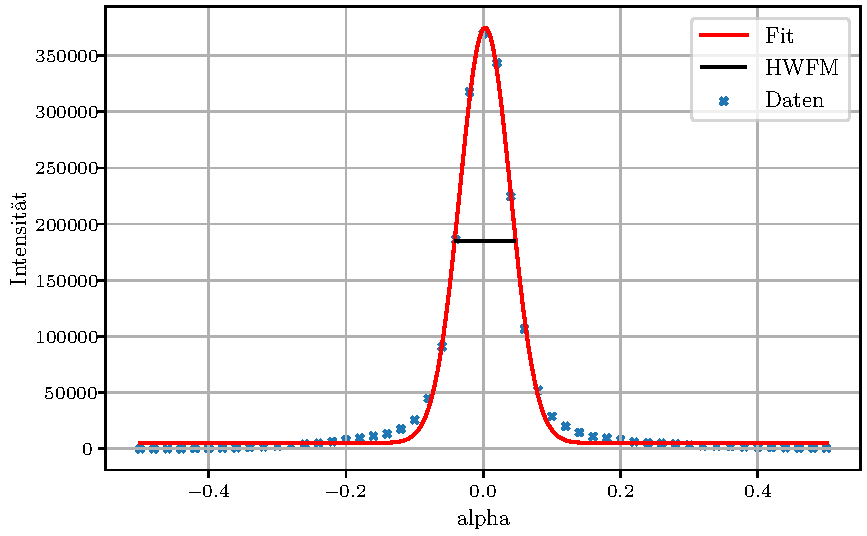
\includegraphics[width=\textwidth]{plots/detectorscan.pdf}
    \caption{Detektorscan mit Gaußfit und HWFM-Linie.}
    \label{fig:detektorscan}
\end{figure}

Die Fitparameter berechnen sich zu

\begin{align*}
    \mu &= \qty{0.0026(4)}{\degree} \\
    \sigma &= \qty{0.0369(4)}{\degree} \\
    a &= \num{34247(410)} \\
    b &= \num{5197(917)}.
\end{align*}

Das Maximum befindet sich bei ungefähr
\begin{equation*}
    I_\text{max} = \num{369567(329)}
\end{equation*}
und die Grenzen der vollen Breite bei halbem Maximum (FWHM) liegen bei ungefähr
\begin{align*}
   \text{HWFM}_\text{links} &= \qty{-0.041}{\degree} \\
   \text{HWFM}_\text{rechts} &= \qty{0.046}{\degree}.
\end{align*}

\subsection{Geometrie des Strahls}

Die Strahlbreite wird über den Z-Scan ermittelt, zu sehen in \autoref{fig:strahlbreite}.

\begin{figure}[H]
    \centering
    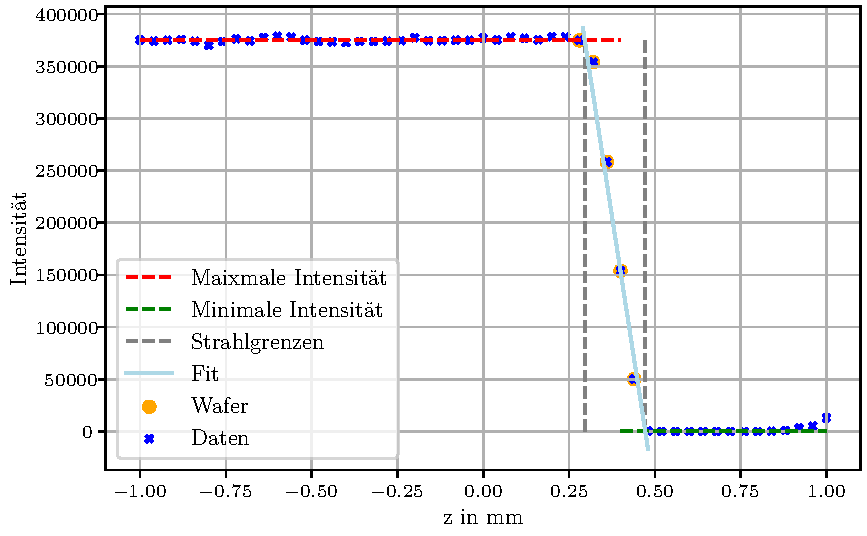
\includegraphics[width=\textwidth]{plots/zscan.pdf}
    \caption{Z-Scan des Strahls. Die volle Intensität, wenn der Strahl nicht geblockt wird, und die minimale Intensität, wenn der Strahl komplett geblockt ist, sind über Mittelwerte dargestellt.
    Die Intensitätsabnahme des Strahls wird linear genähert und die Grenzen markiert.}
    \label{fig:strahlbreite}
\end{figure}

Die Intensitäten werden genähert mit
\begin{align*}
    I_\text{volle Intensität} &= \qty{374812(344)}{} \\
    I_\text{minimale Intensität} &= \qty{399(23)}{} \\
    I_\text{Strahl}(\alpha) &= \qty{-2123867(241153)}{\per\degree} \cdot \alpha + \qty{1002844(87880)}{}.
\end{align*}

Die Lasergrenzen liegen somit bei
\begin{align*}
    \alpha_\text{Linke Grenze} &= \qty{0.295(18)}{\milli\meter} \\
    \alpha_\text{Rechte Grenze} &= \qty{0.471(25)}{\milli\meter},
\end{align*}

was einer Strahlbreite von 
\begin{equation*}
    d = \qty{0.176(30)}{\milli\meter}
\end{equation*}

entspricht. 

Der Geometriewinkel wird einmal berechnet und anschließend gemessen. Nach \autoref{eq:geometriewinkel}
ergibt sich mit der Strahlbreite $d$ ein theoretischer Geometriewinkel von
\begin{equation*}
    \alpha_\text{g, theo.} = \qty{0.51(9)}{\degree}.
\end{equation*}

Mit dem Rockingscan in \autoref{fig:rockingscan} kann der Geometriewinkel gemessen werden.

\begin{figure}[H]
    \centering
    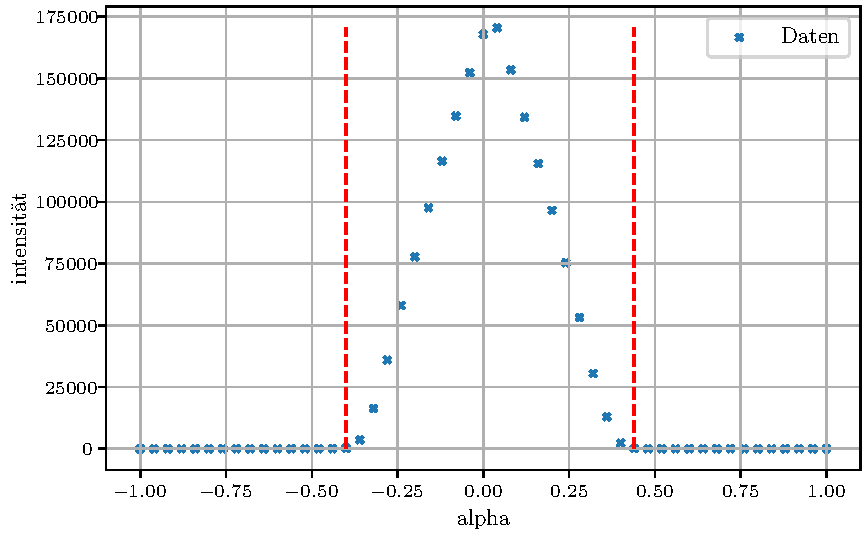
\includegraphics[width=\textwidth]{plots/rockingscan.pdf}
    \caption{Rockingscan zur Bestimmung des Geometriewinkels, angedeutet mit gestrichelten Linien.}
    \label{fig:rockingscan}
\end{figure}

Die Nulldurchgänge liegen hier bei $\alpha_{0\text{, links}} = \qty{-0.4}{\degree}$ und $\alpha_{0\text{, rechts}} = \qty{0.44}{\degree}$.
Der mittlere Geometriewinkel liegt in der Messung bei 
\begin{equation*}
    \alpha_\text{g, mess.} = \qty{0.42(2)}{\degree}
\end{equation*}

\subsection{Reflektivität}

Es wird ein Reflektivitätsscan und ein diffuser Scan aufgenommen, zu sehen in \autoref{fig:reflectivity}. Auf der $y$-Achse sind nicht die direkten Messwerte dargestellt, sondern die Reflektivitätsscan
\begin{equation*}
    R = \frac{I_\text{Mess}}{5\cdot I_\text{Max}},
\end{equation*}
wobei der Faktor $5$ im Nenner dadurch begründet ist, dass das Maximum in \autoref{fig:detektorscan} nur über $1$ Sekunde aufgenommen wurde, die Messung der Reflektivität aber über $5$ Sekunden lief.

\begin{figure}[H]
    \centering
    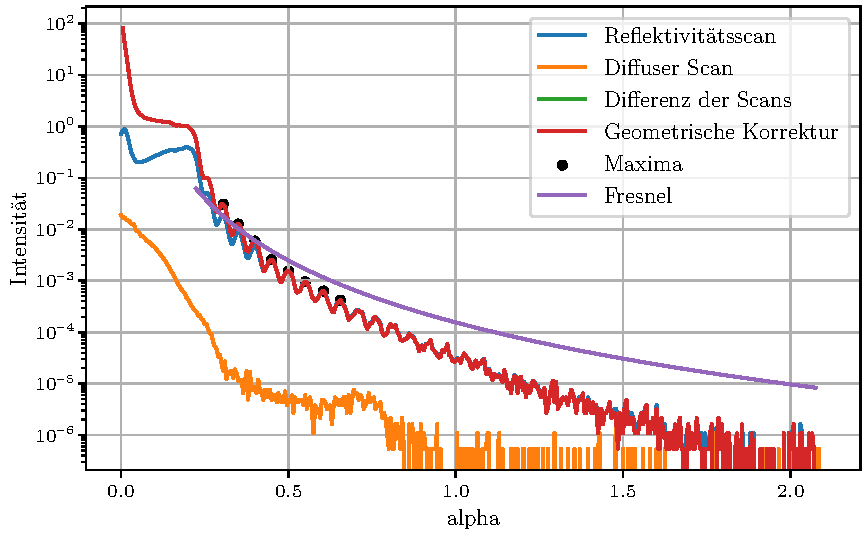
\includegraphics[width=\textwidth]{plots/reflectivity.pdf}
    \caption{Die Messung des Reflektivitätsscans (blau), des diffusen Scans (orange), die Differenz (grün, überdeckt), die Differenz bereinigt um die geometrische Korrektur (rot), ausgewählte Maxima (schwarze Punkte) und die reine Fresnelreflektivität (lila).}
    \label{fig:reflectivity}
\end{figure}

Aus den Abständen aufeinanderfolgender Maxima bzw. Minima lässt sich die Schichtdicke nach \autoref{eq:schichtdicke} abschätzen zur
\begin{equation*}
    d = \qty{8.83(25)e-8}{\meter},
\end{equation*}

die dafür herangezogenen Maxima sind ebenfalls in \autoref{fig:reflectivity} dargestellt.

Mit dem Parratt-Algorithmus \ref{eq:parratt} kann die Reflektivität genähert werden. Um die nötigen Parameter zu bestimmen,
wird eine Parametersuche mit optuna gemacht. Die gefundenen Parameter sind dargestellt in \autoref{tab:parratt}.

\begin{table}[H]
    \centering
    \caption{Gefundene Parratt-Parameter.}
    \label{tab:parratt}
    \begin{tabular}{c c}
        \toprule
        {Parameter} & {Wert} \\
        \midrule
        Schichtdicke & $\qty{8.693e-8}{\meter}$ \\
        $\delta_\text{Si}$ & $\num{7.861e-6}$ \\
        $\delta_\text{Poly}$ & $\num{9.418e-7}$ \\
        $\beta_\text{Si}$    & $\num{8.645e-8}$ \\
        $\beta_\text{Poly}$  & $\num{1.405e-8}$ \\
        $\sigma_\text{Si}$   & $\qty{5.182e-10}{\meter}$ \\
        $\sigma_\text{Poly}$ & $\qty{9.966e-10}{\meter}$ \\
        \bottomrule
    \end{tabular}
\end{table}

Die Näherung durch den Parratt-Algorithmus ist dargestellt in \autoref{fig:parratt}.

\begin{figure}[H]
    \centering
    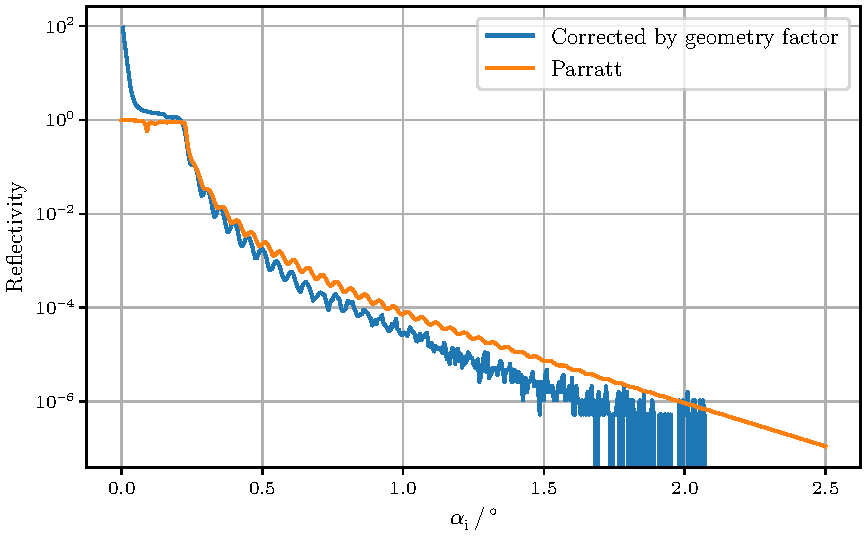
\includegraphics[width=\textwidth]{plots/parrat_comparison.pdf}
    \caption{Korrigierte Messdaten und Parratt-Algorithmus.}
    \label{fig:parratt}
\end{figure}

Die Parameter des Parratt-Algorithmus ergeben mit \autoref{eq:kritischerwinkel} kritische Winkel von

\begin{align*}
    \theta_\text{c, Si} &= \qty{0.227}{\degree} \\
    \theta_\text{c, Poly} &= \qty{0.078}{\degree}.
\end{align*}

